\documentclass[11pt]{article}

\usepackage{times}
\usepackage{epsf}
\usepackage{epsfig}
\usepackage{amsmath, alltt, amssymb, xspace}
\usepackage{wrapfig}
\usepackage{fancyhdr}
\usepackage{url}
\usepackage{verbatim}
\usepackage{fancyvrb}

\usepackage{subfigure}
\usepackage{cite}
%\usepackage{cases}
%\usepackage{ltexpprt}
%\usepackage{verbatim}

%\topmargin      -0.70in  % distance to headers
%\headheight     0.2in   % height of header box
%\headsep        0.4in   % distance to top line
%\footskip       0.3in   % distance from bottom line

% Horizontal alignment
\topmargin      -0.50in  % distance to headers
\oddsidemargin  0.0in
\evensidemargin 0.0in
\textwidth      6.5in
\textheight     8.9in 


%\centerfigcaptionstrue

%\def\baselinestretch{0.95}


\newcommand\discuss[1]{\{\textbf{Discuss:} \textit{#1}\}}
%\newcommand\todo[1]{\vspace{0.1in}\{\textbf{Todo:} \textit{#1}\}\vspace{0.1in}}
\newtheorem{problem}{Problem}[section]
%\newtheorem{theorem}{Theorem}
%\newtheorem{fact}{Fact}
\newtheorem{define}{Definition}[section]
%\newtheorem{analysis}{Analysis}
\newcommand\vspacenoindent{\vspace{0.1in} \noindent}

%\newenvironment{proof}{\noindent {\bf Proof}.}{\hspace*{\fill}~\mbox{\rule[0pt]{1.3ex}{1.3ex}}}
%\newcommand\todo[1]{\vspace{0.1in}\{\textbf{Todo:} \textit{#1}\}\vspace{0.1in}}

%\newcommand\reducespace{\vspace{-0.1in}}
% reduce the space between lines
%\def\baselinestretch{0.95}

\newcommand{\fixmefn}[1]{ \footnote{\sf\ \ \fbox{FIXME} #1} }
\newcommand{\todo}[1]{
\vspace{0.1in}
\fbox{\parbox{6in}{TODO: #1}}
\vspace{0.1in}
}

\newcommand{\mybox}[1]{
\vspace{0.2in}
\noindent
\fbox{\parbox{6.5in}{#1}}
\vspace{0.1in}
}


\newcounter{question}
\setcounter{question}{1}

\newcommand{\myquestion} {{\vspace{0.1in} \noindent \bf Question \arabic{question}:} \addtocounter{question}{1} \,}

\newcommand{\myproblem} {{\noindent \bf Problem \arabic{question}:} \addtocounter{question}{1} \,}


\newcommand{\copyrightnoticeA}[1]{
\vspace{0.1in}
\fbox{\parbox{6in}{\small Copyright \copyright\ 2006 - 2014\ \ Wenliang Du, Syracuse University.\\ 
      The development of this document is partially funded by 
      the National Science Foundation's Course, Curriculum, and Laboratory 
      Improvement (CCLI) program under Award No. 0618680 and 0231122. 
      Permission is granted to copy, distribute and/or modify this document
      under the terms of the GNU Free Documentation License, Version 1.2
      or any later version published by the Free Software Foundation.
      A copy of the license can be found at http://www.gnu.org/licenses/fdl.html.}}
\vspace{0.1in}
}


\newcommand{\copyrightnotice}[1]{
\vspace{0.1in}
\fbox{\parbox{6in}{\small Copyright \copyright\ 2006 - 2014\ \ Wenliang Du, Syracuse University.\\
      The development of this document is/was funded by three grants from
      the US National Science Foundation: Awards No. 0231122 and 0618680 from
      TUES/CCLI and  Award No. 1017771 from Trustworthy Computing.
      This lab was imported into the Labtainer framework by the Naval Postgraduate 
      School, Center for Cybersecurity and Cyber Operations under National Science 
      Foundation Award No. 1438893.
      Permission is granted to copy, distribute and/or modify this document
      under the terms of the GNU Free Documentation License, Version 1.2
      or any later version published by the Free Software Foundation.
      A copy of the license can be found at http://www.gnu.org/licenses/fdl.html.}}
\vspace{0.1in}
}

\newcommand{\copyrightnoticeB}[1]{
\vspace{0.1in}
\fbox{\parbox{6in}{\small Copyright \copyright\ 2006 - 2014\ \ Wenliang Du, Syracuse University.\\
      The development of this document is/was funded by the following grants from
      the US National Science Foundation: No. 0231122, 0618680, and 1303306.
      Permission is granted to copy, distribute and/or modify this document
      under the terms of the GNU Free Documentation License, Version 1.2
      or any later version published by the Free Software Foundation.
      A copy of the license can be found at http://www.gnu.org/licenses/fdl.html.}}
\vspace{0.1in}
}


\newcommand{\nocopyrightnotice}[1]{
\vspace{0.1in}
\fbox{\parbox{6in}{\small  
      The development of this document is funded by 
      the National Science Foundation's Course, Curriculum, and Laboratory 
      Improvement (CCLI) program under Award No. 0618680 and 0231122. 
      Permission is granted to copy, distribute and/or modify this document.
      }}
\vspace{0.1in}
}

\newcommand{\idea}[1]{
\vspace{0.1in}
{\sf IDEA:\ \ \fbox{\parbox{5in}{#1}}}
\vspace{0.1in}
}

\newcommand{\questionblock}[1]{
\vspace{0.1in}
\fbox{\parbox{6in}{#1}}
\vspace{0.1in}
}


\newcommand{\minix}{{\tt Minix}\xspace}
\newcommand{\unix}{{\tt Unix}\xspace}
\newcommand{\linux}{{\tt Linux}\xspace}
\newcommand{\ubuntu}{{\tt Ubuntu}\xspace}
\newcommand{\selinux}{{\tt SELinux}\xspace}
\newcommand{\freebsd}{{\tt FreeBSD}\xspace}
\newcommand{\solaris}{{\tt Solaris}\xspace}
\newcommand{\windowsnt}{{\tt Windows NT}\xspace}
\newcommand{\setuid}{{\tt Set-UID}\xspace}
%\newcommand{\smx}{{\tt Smx}\xspace}
\newcommand{\smx}{{\tt Minix}\xspace}
\newcommand{\relay}{{\tt relay}\xspace}
\newcommand{\isys}{{\tt iSYS}\xspace}
\newcommand{\ilan}{{\tt iLAN}\xspace}
\newcommand{\iSYS}{{\tt iSYS}\xspace}
\newcommand{\iLAN}{{\tt iLAN}\xspace}
\newcommand{\iLANs}{{\tt iLAN}s\xspace}
\newcommand{\bochs}{{\tt Bochs}\xspace}

\newcommand\FF{{\mathcal{F}}}

\newcommand{\argmax}[1]{
\begin{minipage}[t]{1.25cm}\parskip-1ex\begin{center}
argmax
#1
\end{center}\end{minipage}
\;
}

\newcommand{\bm}{\boldmath}
\newcommand  {\bx}    {\mbox{\boldmath $x$}}
\newcommand  {\by}    {\mbox{\boldmath $y$}}
\newcommand  {\br}    {\mbox{\boldmath $r$}}


%\pagestyle{fancyplain}
%\lhead[\thepage]{\thesection}      % Note the different brackets!
%\rhead[\thesection]{SEED Laboratories}
%\lfoot[\fancyplain{}{}]{Syracuse University} 
%\cfoot[\fancyplain{}{}]{\thepage} 

\newcommand{\tstamp}{\today}   
%\lhead[\fancyplain{}{\thepage}]         {\fancyplain{}{\rightmark}}
%\chead[\fancyplain{}{}]                 {\fancyplain{}{}}
%\rhead[\fancyplain{}{\rightmark}]       {\fancyplain{}{\thepage}}
%\lfoot[\fancyplain{}{}]                 {\fancyplain{\tstamp}{\tstamp}}
%\cfoot[\fancyplain{\thepage}{}]         {\fancyplain{\thepage}{}}
%\rfoot[\fancyplain{\tstamp} {\tstamp}]  {\fancyplain{}{}}

\pagestyle{fancy}
%\lhead{\bfseries Computer Security Course Project}
\lhead{\bfseries SEED Labs}
\chead{}
\rhead{\small \thepage}
\lfoot{}
\cfoot{}
\rfoot{}

\usepackage{listings}
\usepackage{color}

\definecolor{dkgreen}{rgb}{0,0.6,0}
\definecolor{gray}{rgb}{0.5,0.5,0.5}
\definecolor{mauve}{rgb}{0.58,0,0.82}

\lstset{frame=tb,
  language=C,
  aboveskip=3mm,
  belowskip=3mm,
  showstringspaces=false,
  columns=flexible,
  basicstyle={\small\ttfamily},
  numbers=none,
  numberstyle=\tiny\color{gray},
  keywordstyle=\color{blue},
  commentstyle=\color{dkgreen},
  stringstyle=\color{mauve},
  breaklines=true,
  breakatwhitespace=true,
  tabsize=3
}



\begin{document}

\begin{center}
{\LARGE DMZ Lab}
\vspace{0.1in}\\
\end{center}

\copyrightnotice

\section{Overview}
This lab requires that you configure a DMZ using iptables on two gateway components.

\section{Lab Environment}
This lab runs in the Labtainer framework,
available at http://my.nps.edu/web/c3o/labtainers.
That site includes links to a pre-built virtual machine
that has Labtainers installed, however Labtainers can
be run on any Linux host that supports Docker containers.

From your labtainer-student directory start the lab using:
\begin{verbatim}
    labtainer dmz-lab
\end{verbatim}
\noindent A link to this lab manual will be displayed.  

\section{Network Configuration}
This lab includes several networked computers as shown in Figure~\ref{fig:topology}.
Note however that your instance of the lab will have different IP addresses
for some of the components.
When the lab starts, you will get several virtual terminals, one connected to each
component.

The outer gateway and the remote gateway each reach the Internet via an ISP with 
address 198.18.0.1.  The local site has a network address of 198.18.1.0/24.  The remote
site has a network address of 203.0.113.0/24.

Initially, the DMZ is in name only.  For example, there is nothing stopping the 
remote workstation from pinging the ws1.

\begin{figure}[H]
\begin{center}
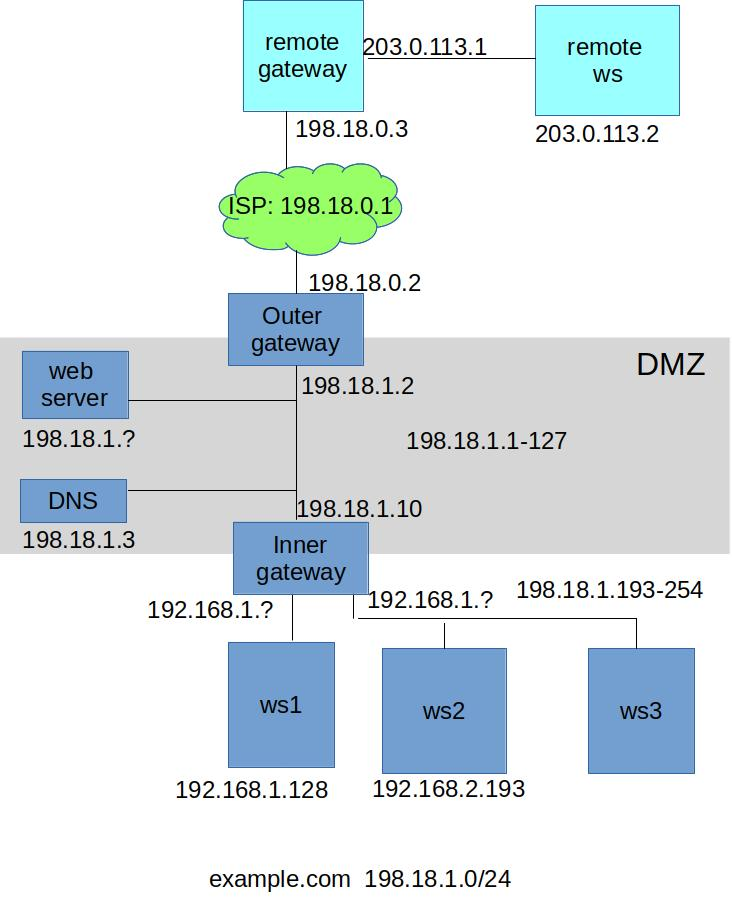
\includegraphics [width=0.8\linewidth]{dmz-lab.jpg}
\end{center}
\caption{Network topology for dmz-lab}
\label{fig:topology}
\end{figure}

\section{Lab Tasks}
\subsection{Explore}
Use the different terminals to test your ability to reach different computers.
The nmap utility is installed on the workstations.  
\subsection{Configure the DMZ}
Configure the inner\_gateway and outer\_gateway such that:
\begin{itemize}
\item Remote users can only access the web server, e.g., via wget www.example.com, using
HTTP, HTTPS and SSH.
\item Remove users cannot access any of the other local computers.
\item Local users can reach the internet via the ISP, e.g., wget www.google.com
\item Local users can reach the local web server via HTTP, HTTPS, SSH and MYSQL
\end{itemize}

Use the /etc/rc.local scripts on the inner and outer gateways to issue iptables directives.
Respect the comments in the rc.local scripts regarding sections that should not be modified.
Consider using NAT to isolate the local workstations from the Internet (there is no reason
for workstations to be addressable from outside of example.com.

\subsection{Demonstrate your DMZ}
Demonstrate your DMZ by issuing the following commands, without any additional changes to iptables.
\begin{enumerate}
\item On the remote\_ws (hank): {\tt sudo nmap www.example.com}
\item On the ws1 (tom): {\tt sudo nmap www.example.com}
\item On the ws1 (tom): {\tt wget www.google.com}
\end{enumerate}
\noindent If you make any changes to iptables in the course of your testing, restart your testing from
item (1) above.

\subsection{Check your work}
Use the {\tt checkwork} command from the terminal at which you started the lab.  This will provide
feedback informing you of any problems found with your DMZ.

\section{Submission}
After finishing the lab, go to the terminal on your Linux system that was used to start the lab and type:
\begin{verbatim}
    stoplab dmz-lab
\end{verbatim}
When you stop the lab, the system will display a path to the zipped lab results on your Linux system.  Provide that file to 
your instructor, e.g., via the Sakai site.

\end{document}
